\section{Apprentissage}

\subsection{D\'efinitions : epoch, step, batch}
Conform\'ement au cours, l'apprentissage supervis\'e du CNN de la Section~III consiste \`a ajuster un ensemble de poids entra\^inables
\begin{equation}
W=\{w_{ij}\},
\end{equation}
sur l'ensemble d'apprentissage $A=\{(X_i,V_i)\}_{i=1}^{N}$, de mani\`ere \`a minimiser la loss empirique
\begin{equation}
\begin{aligned}
L_A(W)
&=
\frac{1}{N}
\sum_{i=1}^{N}
L\!\left(\mathrm{ForwardProp}(W,X_i),V_i\right),\\
\widehat{W}
&=
\arg\min_{W} L_A(W).
\end{aligned}
\label{eq:section4_training_objective}
\end{equation}
Lorsque $A$ est partitionn\'e en lots $A_b\subset A$, $|A_b|=B$, la loss associ\'ee \`a un lot est d\'efinie par
\begin{equation}
L_b(W)
=
\frac{1}{|A_b|}
\sum_{(X_i,V_i)\in A_b}
L\!\left(\mathrm{ForwardProp}(W,X_i),V_i\right).
\label{eq:section4_batch_loss}
\end{equation}
Cette normalisation par $|A_b|$ est retenue dans toute la section, car elle permet de comparer des batch sizes diff\'erents sans modifier artificiellement l'\'echelle num\'erique de la loss ; elle correspond en outre \`a la convention de r\'eduction \texttt{sum\_over\_batch\_size} utilis\'ee dans l'impl\'ementation Keras.

Une it\'eration d'optimisation sur un lot s'\'ecrit alors, pour chaque connexion $(i,j)$,
\begin{equation}
w_{ij}^{(t)} = w_{ij}^{(t-1)} - \epsilon \, \frac{\partial L_b}{\partial w_{ij}},
\label{eq:section4_batch_update}
\end{equation}
o\`u $\epsilon>0$ d\'esigne le pas d'apprentissage. Dans ce cadre, un \textit{batch} est un sous-ensemble $A_b$ de cardinalit\'e $B$, un \textit{step} est une mise \`a jour de la forme~\eqref{eq:section4_batch_update}, et une \textit{epoch} correspond \`a un parcours complet de la base d'apprentissage. Si $N$ exemples sont trait\'es avec des lots de taille $B$, le nombre de steps par epoch vaut
\begin{equation}
S(B)=\left\lceil\frac{N}{B}\right\rceil.
\label{eq:section4_steps_per_epoch}
\end{equation}
Le cours distingue alors trois r\'egimes~: $B=1$ correspond au gradient stochastique, $B=N$ au gradient par lots complets, et $1<B<N$ \`a l'apprentissage par mini-batches, qui recherche un compromis entre bruit du gradient, co\^ut calculatoire et vitesse de convergence \cite{manzanera_classification_apprentissage,poly_chap4_classifml}.

\subsection{Influence de la taille du batch}
\paragraph{Protocole exp\'erimental.}
La pr\'esente section ne red\'efinit ni les donn\'ees ni l'architecture~: le d\'ecoupage des sous-ensembles et la fonction \texttt{standardize} sont ceux de la Section~II, et le CNN entra\^in\'e est celui de la Section~III. Seuls les param\`etres d'apprentissage sont modifi\'es pour l'\'etude des batch sizes et des optimiseurs.

\begin{table}[htbp]
\centering
\caption{Protocole exp\'erimental de la Section~4.}
\label{tab:section4_protocol}
\resizebox{\linewidth}{!}{%
\begin{tabular}{|l|l|}
\hline
R\'ef\'erences amont & Section~II pour les donn\'ees et la standardisation ; Section~III pour l'architecture \\
\hline
Sous-ensembles utilis\'es & $5000$ images d'entra\^inement, $1000$ images de validation ; l'ensemble de test n'intervient pas dans cette section \\
\hline
Graine de partition & $42$ \\
\hline
Graines d'initialisation & $42$, $314$ \\
\hline
Comparaison des batch sizes & $B \in \{8,16,32,64,128\}$, $8$ epochs fixes, SGD avec $\epsilon=10^{-2}$ \\
\hline
Comparaison des optimiseurs & $B=32$, $8$ epochs fixes, m\^emes poids initiaux pour une m\^eme graine \\
\hline
Hyperparam\`etres optimiseurs & SGD~: $\epsilon=10^{-2}$ ; SGD+Momentum~: $\epsilon=10^{-2}$, $\beta=0.9$ ; Adam~: $\epsilon=10^{-3}$, $\beta_1=0.9$, $\beta_2=0.999$, $\eta=10^{-7}$ \\
\hline
Conventions temporelles & temps/step~: moyenne des temps mur mesur\'es sur les lots d'entra\^inement ; temps/epoch~: temps mur d'une epoch incluant la validation \\
\hline
\end{tabular}%
}
\end{table}

La comparaison de la taille du batch est conduite \`a nombre d'epochs fix\'e, et non \`a nombre de mises \`a jour fix\'e. Ce point est essentiel pour l'interpr\'etation~: sur $8$ epochs, le nombre total d'updates vaut $8S(B)$, soit $5000$, $2504$, $1256$, $632$ et $320$ pour $B=8$, $16$, $32$, $64$ et $128$. Les diff\'erences observ\'ees entre batch sizes combinent donc deux effets~: la variation de bruit du gradient et la variation du nombre total de mises \`a jour.

Dans le tableau~\ref{tab:section4_batch_timing}, le symbole $m\pm\sigma$ d\'esigne la moyenne empirique $m$ et l'\'ecart-type empirique $\sigma$~; pour le temps par step, l'agr\'egation porte sur l'ensemble des steps mesur\'es au cours des deux graines et des huit epochs, tandis que pour le temps par epoch elle porte sur l'ensemble des epochs observ\'ees. Les courbes de la figure~\ref{fig:section4_batch_curves} sont les moyennes calcul\'ees sur les deux graines.

\begin{table}[htbp]
\centering
\caption{Influence de la taille du batch sur les co\^uts temporels moyens.}
\label{tab:section4_batch_timing}
\resizebox{\linewidth}{!}{%
\begin{tabular}{|c|c|c|c|}
\hline
Batch size $B$ & Steps/epoch $S(B)$ & Temps moyen par step (s) & Temps moyen par epoch (s) \\
\hline
8 & 625 & 0.0052 $\pm$ 0.0107 & 3.882 $\pm$ 0.460 \\
16 & 313 & 0.0079 $\pm$ 0.0160 & 2.959 $\pm$ 0.391 \\
32 & 157 & 0.0117 $\pm$ 0.0234 & 2.234 $\pm$ 0.410 \\
64 & 79 & 0.0182 $\pm$ 0.0287 & 1.745 $\pm$ 0.371 \\
128 & 40 & 0.0297 $\pm$ 0.0383 & 1.457 $\pm$ 0.340 \\
\hline
\end{tabular}%
}
\end{table}

\begin{figure}[htbp]
\centering
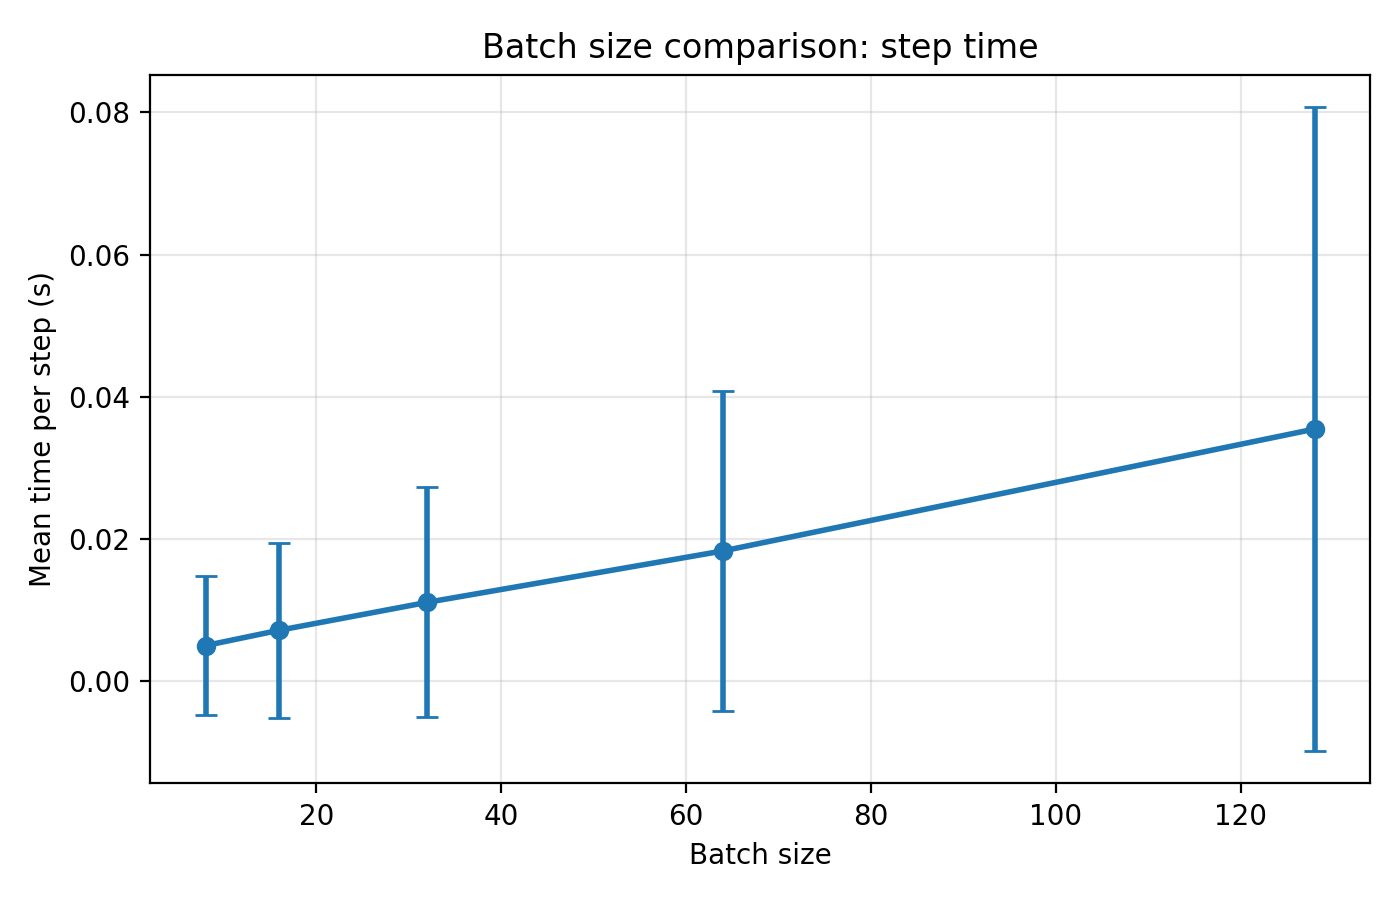
\includegraphics[width=\linewidth]{imgs/section4_batch_step_time.png}
\caption{Temps moyen par step en fonction de la taille du batch.}
\label{fig:section4_batch_step_time}
\end{figure}

\begin{figure}[htbp]
\centering
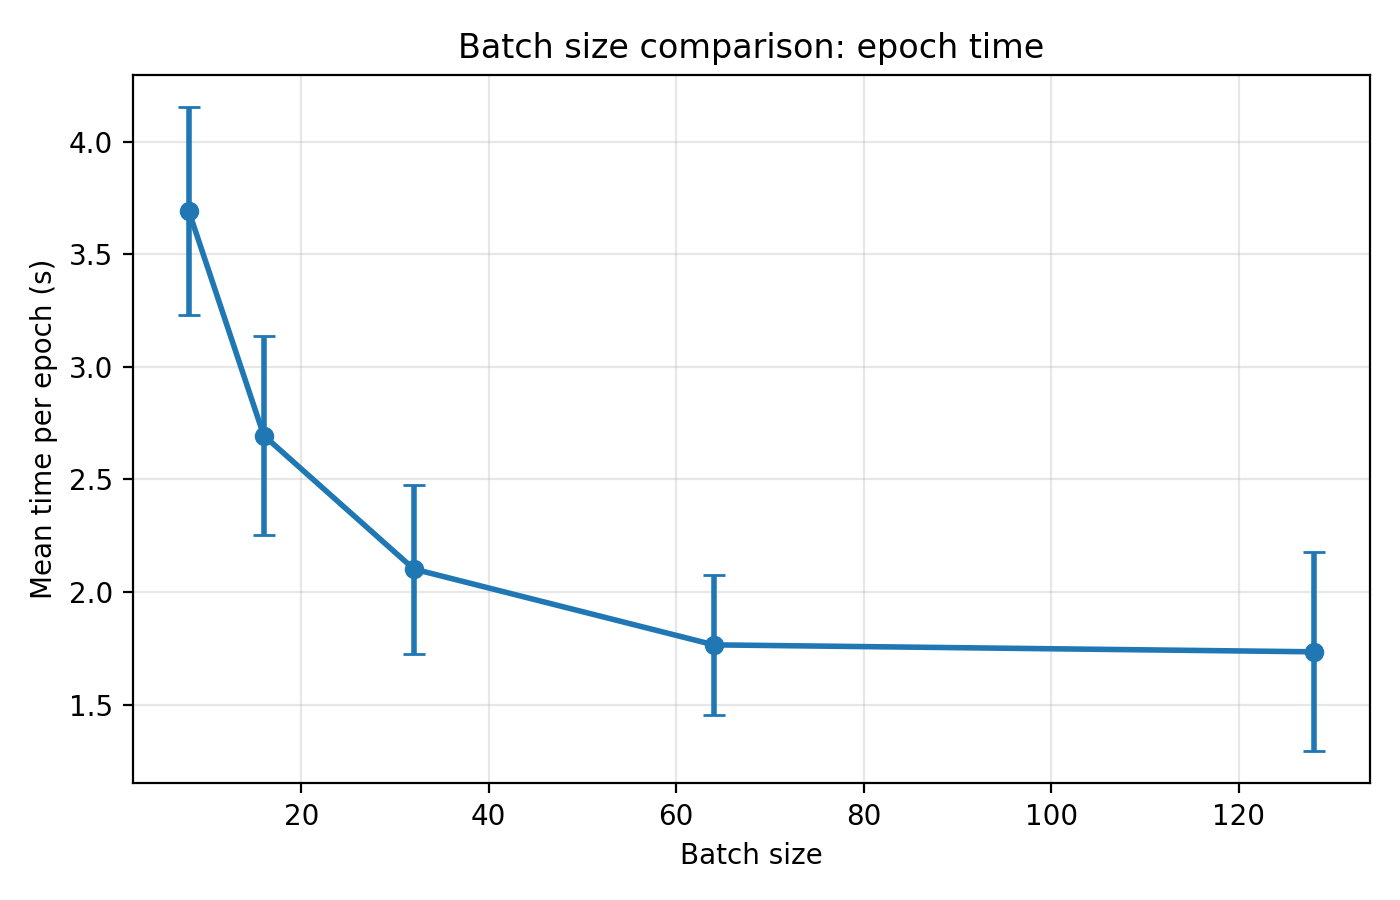
\includegraphics[width=\linewidth]{imgs/section4_batch_epoch_time.png}
\caption{Temps moyen par epoch en fonction de la taille du batch.}
\label{fig:section4_batch_epoch_time}
\end{figure}

Les figures~\ref{fig:section4_batch_step_time} et~\ref{fig:section4_batch_epoch_time} confirment la relation attendue par~\eqref{eq:section4_steps_per_epoch}. Le temps moyen par step cro\^it avec $B$, de $0.0052\,\mathrm{s}$ \`a $0.0297\,\mathrm{s}$, car chaque mise \`a jour traite davantage d'exemples. En sens inverse, le temps moyen par epoch d\'ecro\^it de $3.882\,\mathrm{s}$ \`a $1.457\,\mathrm{s}$, puisque le nombre de steps diminue fortement. Cette d\'ecroissance reste sous-lin\'eaire, ce qui est coh\'erent avec le cours~: l'augmentation de la taille du lot r\'eduit le nombre d'updates mais n'annule pas le surco\^ut de calcul de chaque update \cite{manzanera_classification_apprentissage,poly_chap4_classifml}.

\begin{figure}[htbp]
\centering
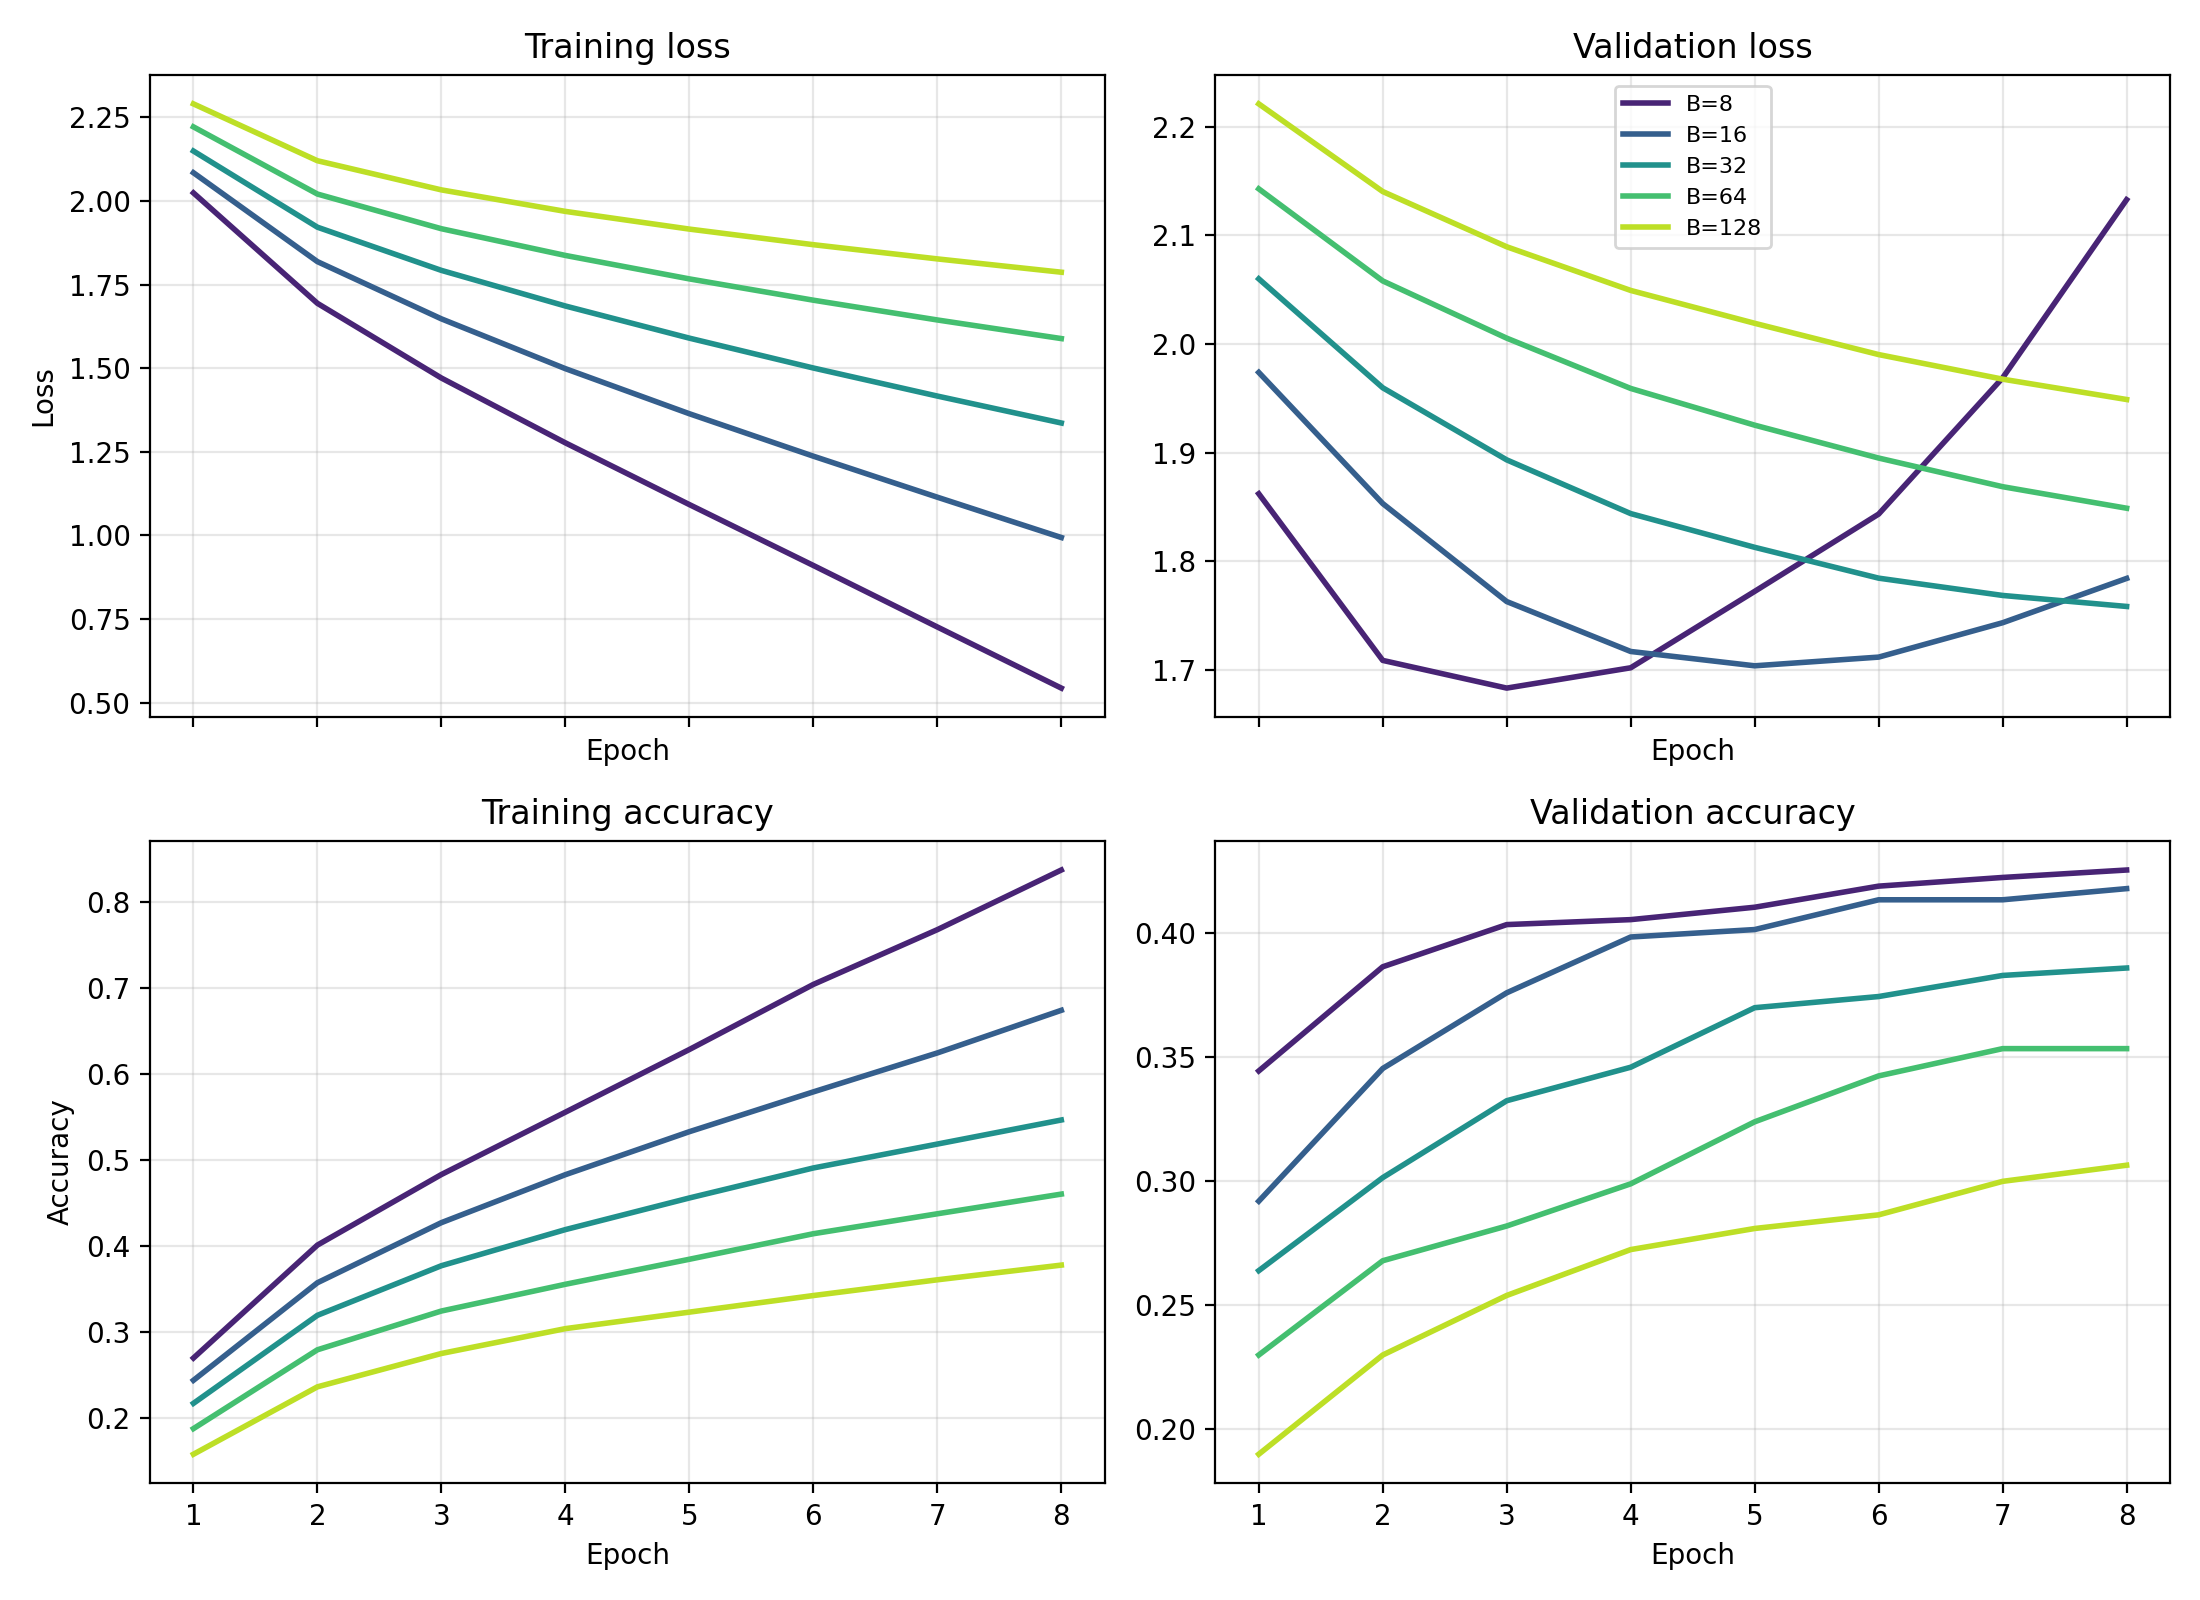
\includegraphics[width=\linewidth]{imgs/section4_batch_curves.png}
\caption{Courbes moyennes d'entra\^inement et de validation pour diff\'erentes tailles de batch.}
\label{fig:section4_batch_curves}
\end{figure}

L'interpr\'etation des courbes doit rester li\'ee au budget fix\'e en epochs. Dans ce cadre, les plus petits batches atteignent les meilleures accuracies de validation finales~: $42.55\%$ pour $B=8$ et $41.80\%$ pour $B=16$, contre $38.60\%$, $35.35\%$ et $30.65\%$ pour $B=32$, $64$ et $128$. Une partie de cet avantage provient du fait que les petits batches r\'ealisent un nombre nettement plus grand de mises \`a jour sur le m\^eme budget de $8$ epochs. En revanche, $B=8$ produit aussi la dynamique de validation la plus bruit\'ee~: la val. loss atteint un minimum moyen de $1.6833$ \`a l'epoch $3$, puis remonte jusqu'\`a $2.1329$ \`a l'epoch $8$. Sous le protocole consid\'er\'e, $B=16$ appara\^it ainsi comme la valeur la plus \'equilibr\'ee parmi celles test\'ees, en conservant une accuracy finale proche de $B=8$ avec des courbes de validation moins irr\'eguli\`eres et un temps par epoch plus faible.

\subsection{Comparaison des m\'ethodes d'optimisation}
Le SGD de base correspond directement \`a l'actualisation scalaire~\eqref{eq:section4_batch_update}, appliqu\'ee \`a chaque connexion $(i,j)$. Le cours pr\'esente ensuite le SGD avec Momentum sous la forme d'une accumulation des gradients successifs~; pour chaque poids $w_{ij}$,
\begin{equation}
G_t = \beta G_{t-1} + (1-\beta)\frac{\partial L_b}{\partial w_{ij}},
\qquad
w_{ij}^{(t)} = w_{ij}^{(t-1)} - \epsilon G_t.
\label{eq:section4_momentum}
\end{equation}
Le terme $G_t$ lisse ainsi les variations de direction du gradient d'un batch au suivant \cite{manzanera_classification_apprentissage,poly_chap4_classifml}.

Pour Adam, la pr\'esente section reprend explicitement l'\'ecriture simplifi\'ee du cours, sans correction de biais~:
\begin{equation}
G_t = \beta_1 G_{t-1} + (1-\beta_1)\frac{\partial L_b}{\partial w_{ij}},
\end{equation}
\begin{equation}
K_t = \beta_2 K_{t-1} + (1-\beta_2)\left(\frac{\partial L_b}{\partial w_{ij}}\right)^2,
\end{equation}
\begin{equation}
w_{ij}^{(t)} = w_{ij}^{(t-1)} - \epsilon \, \frac{G_t}{\sqrt{K_t}+\eta}.
\label{eq:section4_adam}
\end{equation}
Dans cette expression, $\epsilon$ d\'esigne le pas d'apprentissage, tandis que $\eta>0$ est le petit terme introduit au d\'enominateur pour \`eviter une division par z\'ero. Cette m\'ethode adapte donc, pour chaque poids, l'amplitude de la mise \`a jour tout en lissant les fluctuations temporelles du gradient.

La comparaison des optimiseurs est men\'ee \`a batch size fix\'e $B=32$ et \`a nombre d'epochs fix\'e ($8$). Le tableau~\ref{tab:section4_optimizer_summary} regroupe les statistiques agr\'eg\'ees sur les deux graines~; pour le temps par epoch, la notation $m\pm\sigma$ correspond \`a la moyenne et \`a l'\'ecart-type empiriques sur l'ensemble des epochs mesur\'ees, tandis que l'accuracy finale de validation et le minimum de val. loss sont moyenn\'es sur les deux graines.

\begin{table}[htbp]
\centering
\caption{Comparaison des optimiseurs \`a batch size fix\'e $B=32$. Le symbole $\pm$ d\'esigne l'\'ecart-type empirique du temps par epoch.}
\label{tab:section4_optimizer_summary}
\resizebox{\linewidth}{!}{%
\begin{tabular}{|c|c|c|c|}
\hline
Optimiseur & Temps moyen par epoch (s) & Accuracy finale de validation (\%) & Minimum de la val. loss \\
\hline
SGD & 2.133 $\pm$ 0.334 & 38.60 & 1.7584 \\
SGD+Momentum & 2.240 $\pm$ 0.493 & 40.20 & 1.7079 \\
Adam & 2.417 $\pm$ 0.755 & 43.45 & 1.6083 \\
\hline
\end{tabular}%
}
\end{table}

\begin{figure}[htbp]
\centering
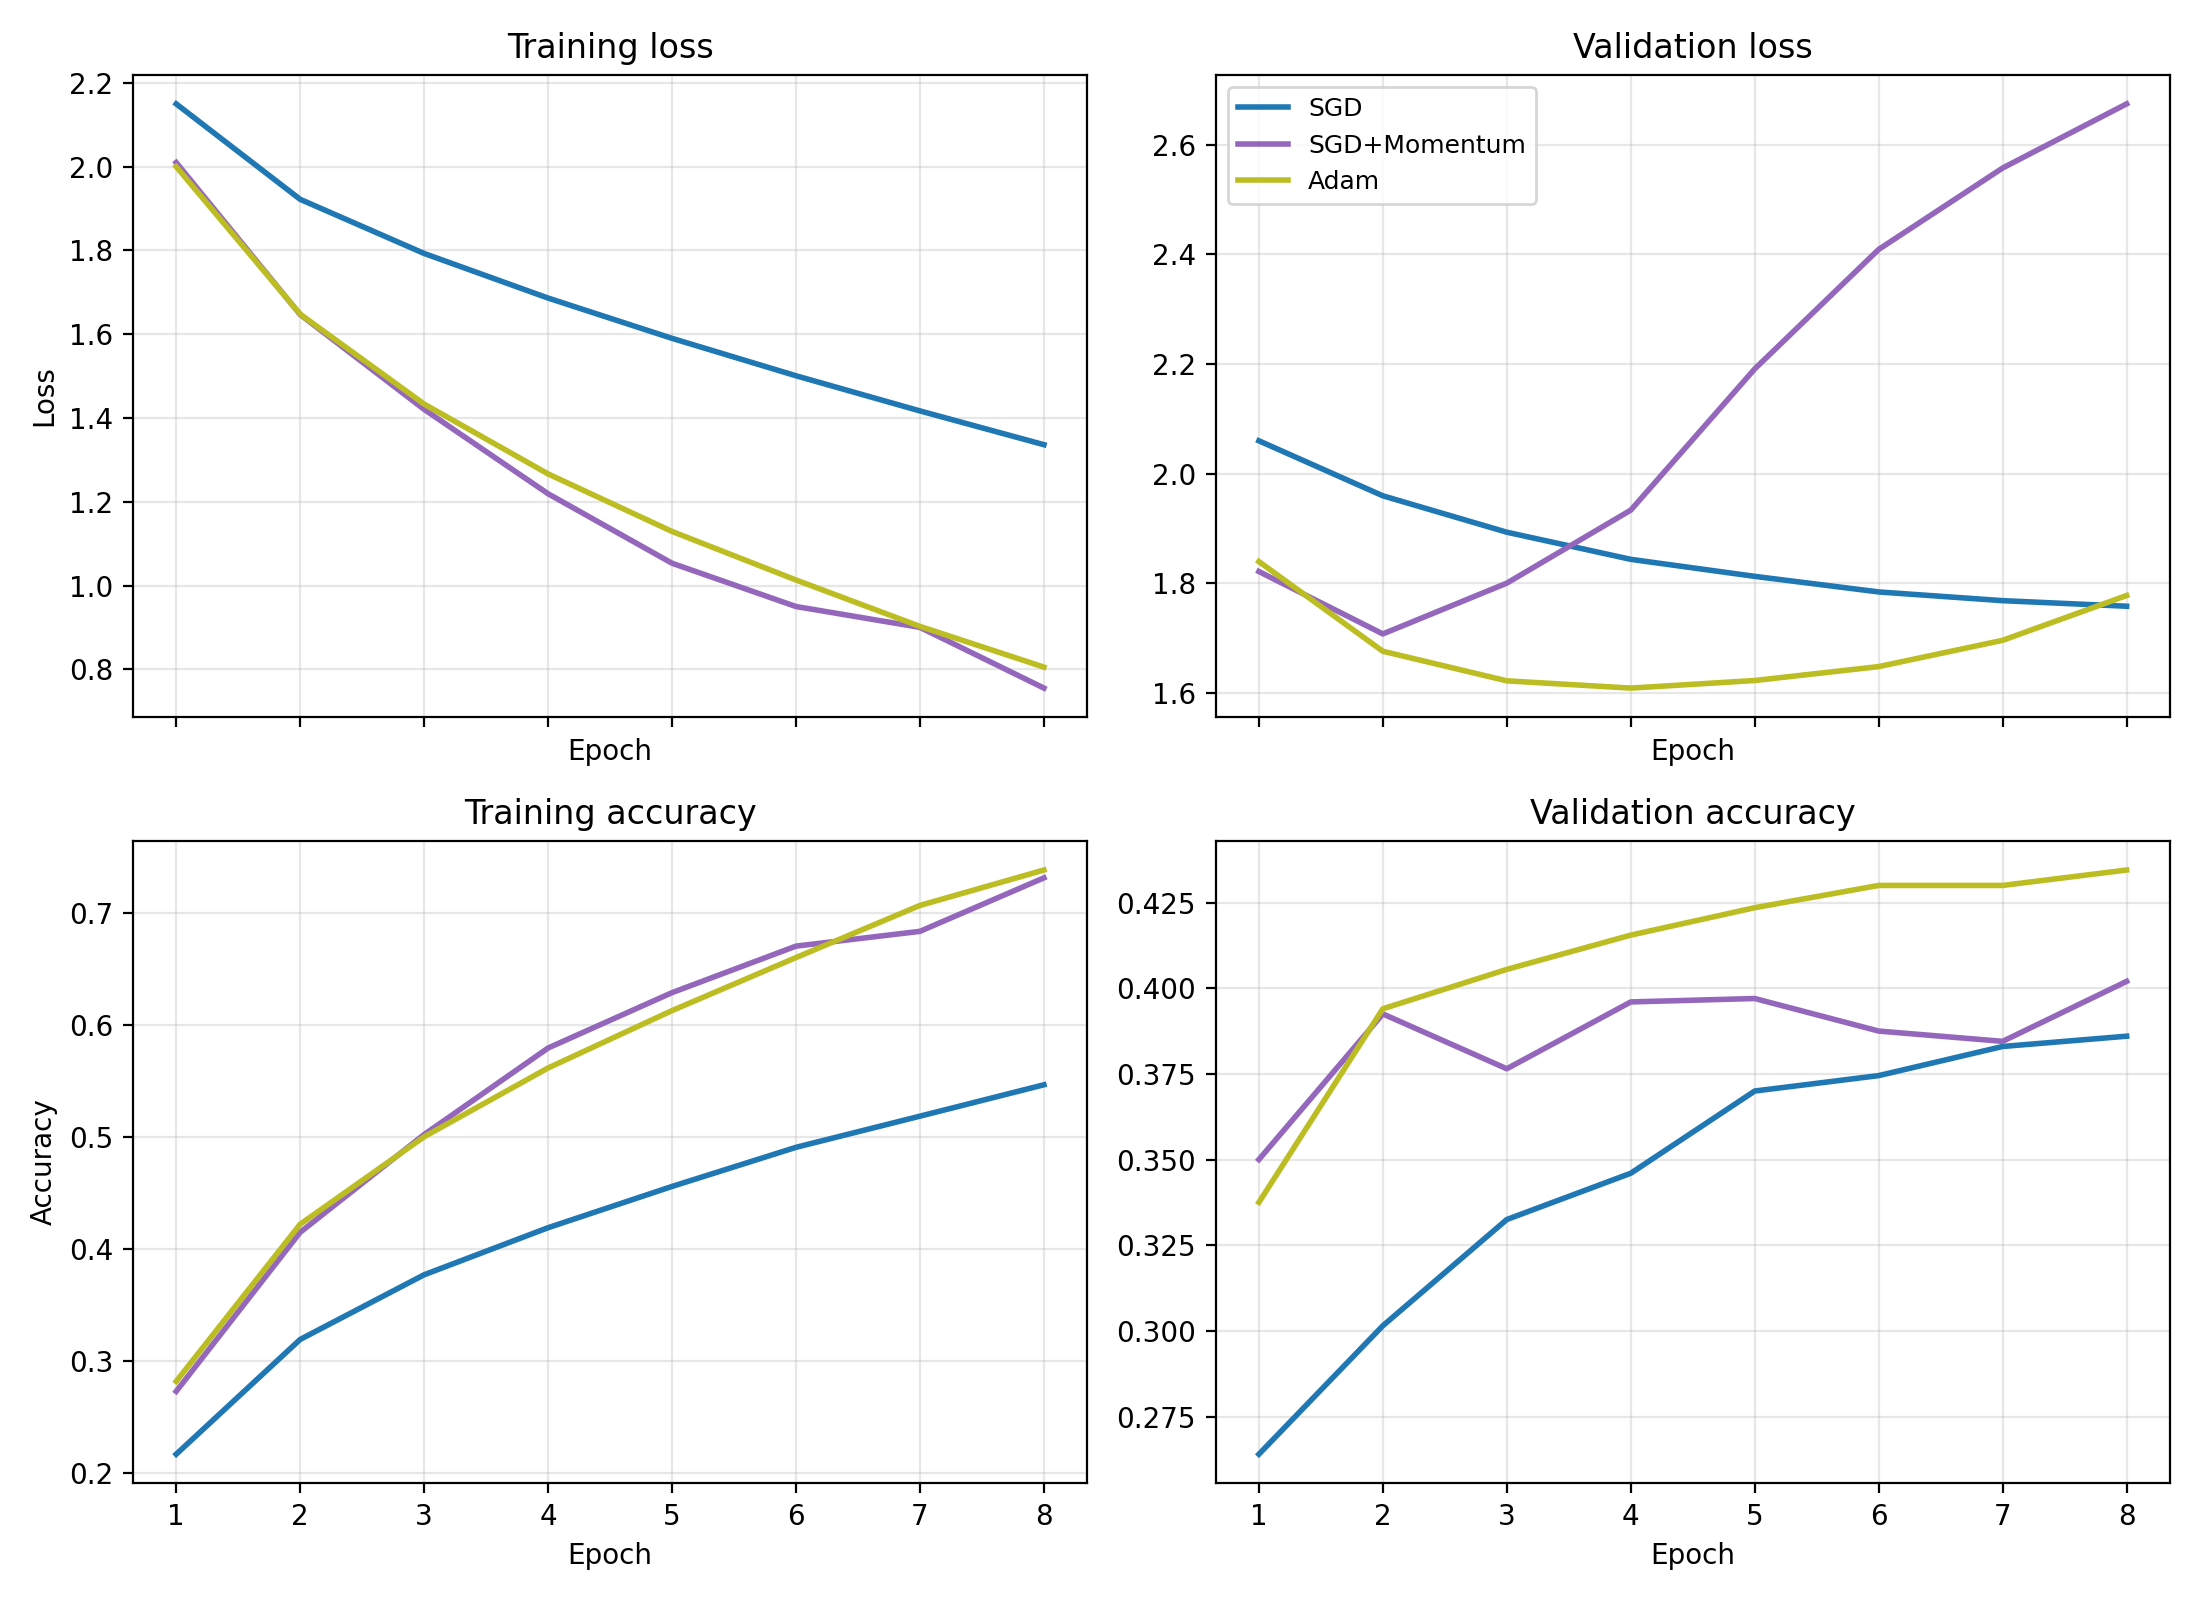
\includegraphics[width=\linewidth]{imgs/section4_optimizer_curves.png}
\caption{Courbes moyennes d'entra\^inement et de validation pour SGD, SGD+Momentum et Adam.}
\label{fig:section4_optimizer_curves}
\end{figure}

Sous ce protocole, le SGD fournit la d\'ecroissance de validation la plus r\'eguli\`ere~: la val. loss baisse presque monotoniquement jusqu'\`a $1.7584$, pour une accuracy finale de $38.60\%$. Le Momentum acc\'el\`ere la descente initiale, avec un minimum moyen de val. loss \`a $1.7079$ d\`es l'epoch $2$, mais la remont\'ee ult\'erieure jusqu'\`a $2.6743$ \`a l'epoch $8$ indique une d\'egradation plus marqu\'ee en fin d'entra\^inement. Cette observation est coh\'erente avec l'interpr\'etation du cours~: le terme $G_t$ stabilise les directions du gradient, mais peut aussi prolonger des mises \`a jour devenues trop agressives lorsque $\epsilon$ reste fix\'e.

Parmi les trois optimiseurs test\'es, Adam obtient les meilleures m\'etriques de validation dans le cadre pr\'esent~: accuracy finale moyenne de $43.45\%$ et minimum moyen de val. loss de $1.6083$. Le surco\^ut temporel reste mod\'er\'e ($2.417\,\mathrm{s}$ par epoch contre $2.133\,\mathrm{s}$ pour SGD), ce qui sugg\`ere que l'adaptation locale des mises \`a jour compense efficacement cette surcharge sur le budget calculatoire consid\'er\'e.

\subsection{Synth\`ese}
Sous le protocole \`a nombre d'epochs fix\'e retenu ici, la taille du batch agit simultan\'ement sur le bruit du gradient et sur le nombre total de mises \`a jour. Les petits batches favorisent donc la performance de validation, mais au prix de courbes plus bruit\'ees et d'un temps par epoch plus \'elev\'e ; parmi les valeurs test\'ees, $B=16$ fournit le compromis le plus favorable entre co\^ut temporel et qualit\'e de validation, tandis que $B=8$ donne l'accuracy finale la plus \'elev\'ee.

\paragraph{Limites exp\'erimentales.}
La port\'ee de ces conclusions reste limit\'ee au protocole \'etudi\'e~: sous-ensemble r\'eduit de CIFAR-10, CNN de taille modeste, apprentissage sur CPU et deux graines d'initialisation seulement. Dans ce cadre, Adam pr\'esente les meilleures m\'etriques de validation parmi les optimiseurs compar\'es, avec un surco\^ut temporel mod\'er\'e ; cette observation ne pr\'etend toutefois pas valoir ind\'ependamment de l'architecture, du budget d'updates ou du choix des hyperparam\`etres.
